\documentclass{article}
\usepackage{amsmath,amssymb,braket,url,hyperref,booktabs,graphicx}
\usepackage[style=nature]{biblatex}
\addbibresource{12_ref.bib}
\newcommand{\bfit}[1]{\textit{\textbf{#1}}}
\begin{document}
\medskip
\noindent
\textbf{\Large Chapter 12\\
Electron Spin Qubit in Semicoductor-1-Qubit and 2-Qubit Gates}\\\\\\
\medskip
\textbf{\large 12.1 Introduction}\\
In Chap.11, we showed how to implement a qubit using electron spin on a silicon
substrate. We also demonetrated how to initialize and measure a qubit. In this chapter,
we will sudy how to perform a universal 1-qubit gate and a 2-qubit entnaglement gate to fulfill
the last two DiVincenzo's criteria (Sect. 1.3). In Chap.10, we showed
that by applying a vertical DC magnetic field and a rotating  horizontal magnetic field and
then \textit{working in the rotating frame}, we would be able to rotate any state on Bloch sphere
about any vector. This allows us to build a universal 1-qubit gate (Section 27.4 in \cite{WongHuiYong})
However, in the literature, many silicon qubits are still implemented with the setup in Chap. 9 which means
that the qubit is places in a vertical DC magnetic field and a perturbating and linearly oscillating horizontal
magnetic field. This is what we will use in this chapter. We will first summarize an experimental paper on how
it implements 1-qubit gate. Then we will discuss the implementation of a 2-qubit entnaglement gate with an example.
\\\\\\
\bfit{\large 12.1.1 Learning Outcomes}
\\\\
Be able to describe how a 1-qubit gate can be implemented for silicon spin qubits; 
understant how a CNOT-gate can be impelmented by using a native entanglement gate of
silicon spin qubits and other 1-qubit gates.
\\\\
\bfit{\large 12.1.2 Teaching Videos}\\\\
$\bullet$ Search for Ch12 in this playlist\\

- \url{https://tinyurl.com/3yhze3jn}\\\\
$\bullet$ Other Videos\\

- \url{https://youtu.be/0JVw4xICV10}

- \url{https://youtu.be/_CpQ-Uy0Kgo}
\\\\\\
\textbf{\large 12.2 1-Qubit Gate Implementation}
\\\\
We will use an example in \cite{veldhorst2014addressable} (with some variation)
to demonstrate how to implement electron spin qubit in silicon and the 1-qubit gate.
The setup is illustrated in Fig. 12.1.

Firstly, the Hilbert space is created by applying a DC magnetic field pointing to the right.
This direction is named the $-\hat{z}$ direction. Therefore, \textit{spin-up means that the spin is 
pointing to the left, and spin-down means that the spin is pointing to the right}. This is nothing
special becuase the name of direction is completely a human definition.

The system is kept at 50 mK and $B_0=1.4T$. This is a spin qubit. To enhance the decoherence
time, we need to avoid the spin interacting with the external environment. The electron spin can
interact with the nuclear spin in the silicon easily and lose its coherence.
Unfortunately, while 95.53\% of natural silicon atoms have a zero nuclear spin
(92.23\% $^{28}Si$ \textbf{isotope} and 3.1\% $^{30}Si$ isotope), 4.67\% of them have
a spin ($^{29}Si$ isotope). This is because $^{29}Si$ has 14 protons and 15 neutrons
and their spins are not nullified due odd number of nucleons. The electron spin will interact
strongly with the nucleus of $^29Si$. Therefore, a highly purified silicon substrate is used,
in which $^29Si$ is reduced to 800 $ppm$ (part-per-million). That means, among 1 million silicon
atoms in the substrate, only 800 will be $^{29}Si$.
\\\\

      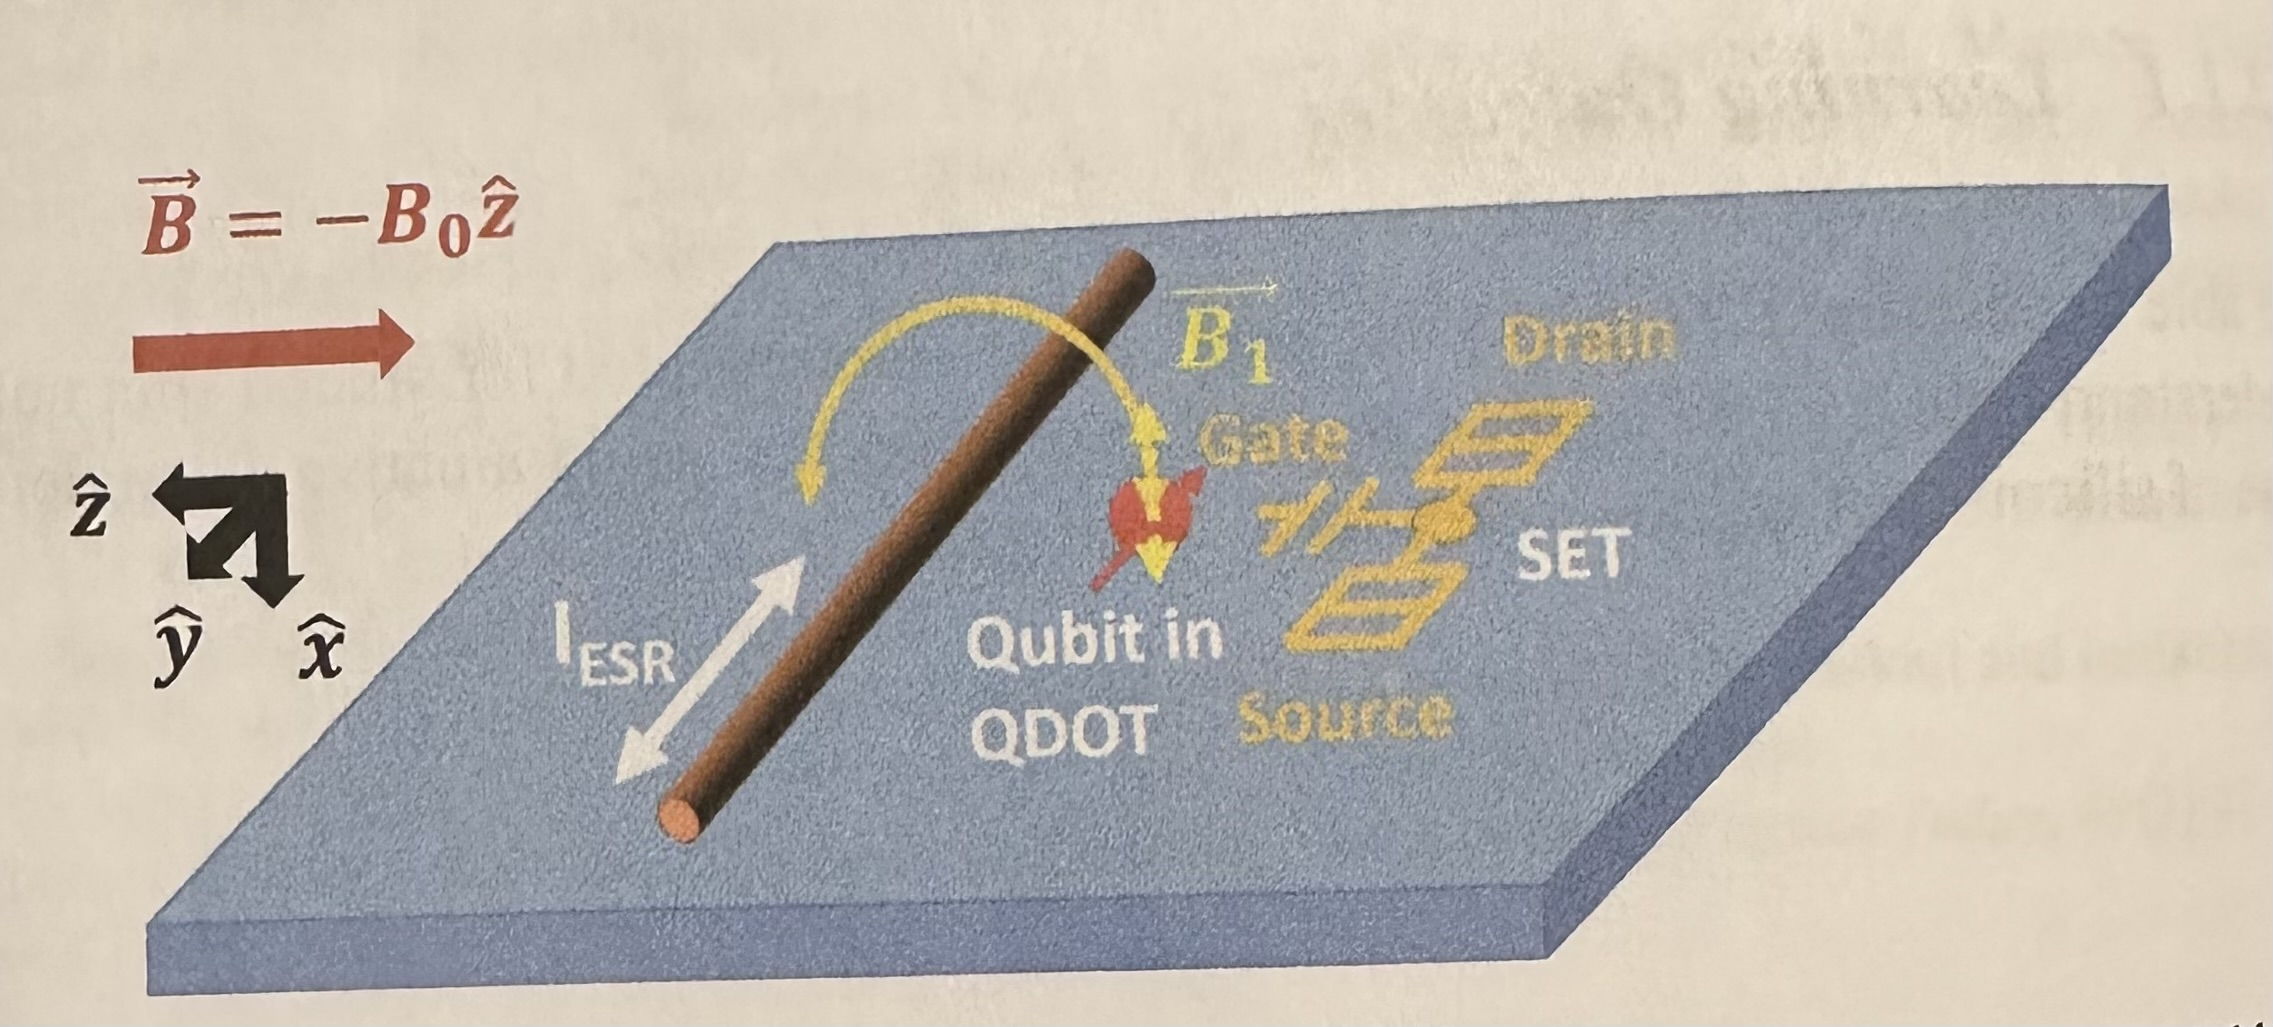
\includegraphics[scale=0.55]{Fig.12.1.jpeg}\\
\textbf{Fig. 12.1} Illustration of how an electron spin qubit is implemented in 
  \cite{veldhorst2014addressable}. The magnetic field due to $I_{ESR}$ is shown and it points
  perpendicular to the substrate at the qubit
\\\\

For \textbf{readout}, it also uses spin-to-charge conversion as in Sect. 11.6. However, instead of using a 
qunatum point contact (QPC) transistor, it uses a \textbf{single electron transistor} (SET) which has its current
also very sensitive to the charge occupation in the quantum dot.

To implement a 1-qubit gate, it uses the theory we learned in Sect 9.3. That is by applying a perturbing oscillating
magnetic field in the $\hat{x}$ direction. But note that, the $\hat{x}$ direaction in Fig.12.1 is perpendicular to the silicon substrate.
To achieve the oscillating magnetic field, an AC electric current, $I_{ESR}$, is passed through
a wire next to the qubit. $ESR$ stands for \textbf{electron spin resonance} which means that its
frequency is the same as the Larmor frequency due to $\vec{B}$ (see Sect.9.4). The current will generate a circular
magnetic field about the wire due to the \textbf{Biot-Savart law} (see
also Example 24.2). Although it is circular, at the point where it touches the qubit, it is pointing
at the tangential direction of the circle and thus it is pointing in the $\hat{x}$ direction and perpendicular
to the Si substrate. Since $I_{ESR}$ in an AC current, the magnetic field at the qubit oscillates up and down
and has the equation form given in the first term of Eq. (9.5). And as discussed in Sect. 9.6, in therotating frame,
any state will rotate about the $\hat{x^\prime}$ due to Rabi oscillation. Combined with Larmor precession, it can be used
to implement any 1-qubit gate.\\\\\\
\textbf{\large 12.3 2-Qubit Gate for Spin Inmplementation}\\\\
A 2-qubit gate is usually much more difficult to implement than a 1-qubit gate. We also need to recall that, to form
a universal set of quantum gates, what we need is not an arbitary 2-qubit gate but an \textbf{entanglement gate}, which 
can be used to create entanglements (see Sect. 4.6). Entanglement is one of the reasons that makes quantum computing superior
to classical computing.

A 2-qubit gate requires the interaction between two qubits and the external excitation under an appropriate Hamiltonian.
It is not difficult to appreciate that different quatum computer architectures have different "native" entnaglement gates because 
the physics is fairly different in different quantum computing archtectures. Here, a \textbf{native entanglement gate} is a gate that 
can be implemented easily using the physics relevant to a given architecture and its controls.

\textit{One of thenative entanglement gates} for an electron spin qubit is a special form of the controlled
phase shift gate. We will call it $\boldsymbol{U_{Cphase}}$ \cite{meunier2011efficient} to distinguish it from 
$\boldsymbol{U_{C P S, \pi}}$ in Section 16.4 in \cite{WongHuiYong},
\begin{equation}\label{eq 12.1}
  \boldsymbol{U_{Cphase}}=\begin{pmatrix}
    1&0&0&0\\0&e^{i\phi}&0&0\\0&0&e^{i(\pi-\phi)}&0\\0&0&0&1
  \end{pmatrix}.\tag{12.1}
\end{equation}
where $\phi$ is the phase. We will discuss how to implement it soon. We will first show how it can be used to create an entanglement.
\\\\\\
\bfit{\large 12.3.1 Creation of Entanglement}
\\\\
We have learned that we can use $C N O T$ gate, $\boldsymbol{U_{XOR}}$ to make two qubits entangled (Section 15.4 in \cite{WongHuiYong} and Sect.4.6). This is
realized with the help of a Hadamard gate, \bfit{H}. This circuit is shown in Fig. 12.2.


\end{document}
